\section{Actividad No 02 – Reconociendo la estructura} 

\begin{enumerate}[1.]
	\item Crear la tabla Departamentos utilizando la siguiente estructura:
	\begin{center}
	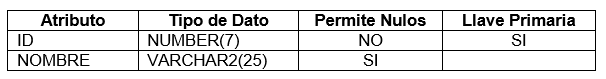
\includegraphics[width=8cm]{./Imagenes/Actividad2} 
	\end{center}
	\item Poblar la tabla Departamentos con los datos de la tabla Departments.
	\item Crear la tabla Empleados utilizando la siguiente estructura.
	\begin{center}
	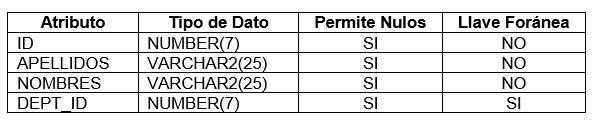
\includegraphics[width=8cm]{./Imagenes/Actividad2_03} 
	\end{center}
	\item Crear la tabla Empleados2 basada en la estructura de la tabla Employees. Incluir solo las columnas EMPLOYEE\_ID, FIRST\_NAME, LAST\_NAME, SALARY y DEPARMENT\_ID 		respectivamente.
	\item Modificar el estado de la tabla Empleados2 a SOLO LECTURA.
	\item Tratar de adicionar el siguiente registro a la tabla Empleados2.
	\begin{center}
	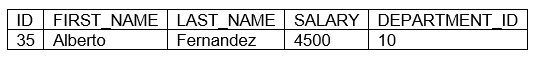
\includegraphics[width=8cm]{./Imagenes/Actividad2_06} 
	\end{center}
	\item Revertir el estado de la tabla LECTURA / ESCRITURA. Tratar de insertar nuevamente la información del punto 4.6.
	\item Eliminar la tabla Empleados2.	
\end{enumerate}